%电子轨道与元素周期表
%未完成:解释一些什么 1s22P2 之类的符号吧!)
在这里, 用最简单的方式介绍原子的壳层结构,并解释元素周期表如何根据壳层结构分出每个周期.

首先画一下原子轨道

为方便画图和描述, 用下图来表示原子, 假设电子的轨道是一个个圆圈.
\begin{figure}[ht]
\centering
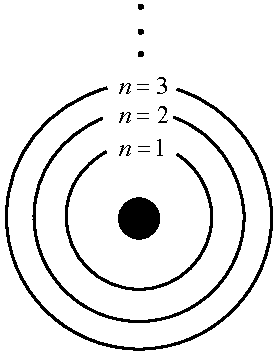
\includegraphics[width=4.5cm]{./figures/Ptable1.pdf}
\caption{电子轨道} 
\end{figure}
现在要把电子放到这些轨道上面来,使电子的总能量最小. 这种状态叫做原子的基态. 理想的状态是,所有电子都在最小的一圈轨道上,但是由于每条轨道只能容纳一定数目的电子,另一些电子不得不进入其他轨道.

为了解释每条轨道能容纳多少电子,把每个轨道的”空位”用一行格子描述. 当一行格子被电子填满时,该轨道就不能容纳更多电子了.
\begin{figure}[ht]
\centering
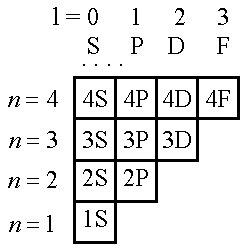
\includegraphics[width=4cm]{./figures/Ptable2.pdf}
\caption{用格子描述电子轨道} 
\end{figure}
给不同的格子命名: 从半径最小的轨道开始,用数字 1,2,3…依次命名每条轨道,这些数字也叫主量子数,用 $n$ 来表示. 在上图中,每条轨道从第一列开始依次用 $S,P,D,F...$ 命名,每一列有相同的角量子数,用 $l$ 来表示.  $S,P,D,F\dots$ 的角量子数依次是 $l = 0,1,2,3\dots$. 把行标和列标组合起来, 就能得到任意一个格子的名称,例如第三行第二列的格子叫做 $3P$. 对于主量子数为 $n$ 的行,角量子数从 0 增加到 $n-1$,也就是说第 $n$ 行有 $n$ 个格子.

接下来,每个格子又能装不同数目的电子,任意一格能装的电子数等于 $(2l + 1) \times 2$. 这是因为,对于角量子数为 $l$ 的格子,还存在另一个参数 $m$,叫磁量子数. 对于特定的角量子数 $l$,$m$ 可以取 $ - l, - l + 1...0,...l - 1,l$ 等 $2l + 1$ 个不同的值. 所以每个格子又可以根据不同的 $m$ 细分成 $2l+1$ 个小格子. 最后, 每一个小格子里面能装两个电子. 总共算下来,第 $n$ 行刚好可以装 $n^2$ 个电子(见下图).

到此为止, 每条轨道承载电子的数目已经解释清楚了, 但是应该如何把电子往格子里面放呢? 为了使电子总能量最小,对于氢原子(1 个核外电子), 显然电子应该放在 $1S$ 格子里, 氦原子(2 个核外电子)可以把两个电子都放在 $1S$ 格子里, 从而把 $n=1$ 的轨道填满, 这就是第一周期的两个原子的电子分布. 对于锂原子(3 个核外电子)可以在氦原子的基础上往 $2S$ 格子里放一个电子… 但奇怪的是, 填电子的顺序并不是从下到上从左到右, 而是如下图中的绿色线条和箭头所示, 即按照 $1S, 2S, 2P, 3S, 3P, 4S, 3D, 4P, 5S…$ 的顺序来填上图的格子. 格子内的数字表示每格能装下的电子数, 即 $(2l + 1) \times 2$.
\begin{figure}[ht]
\centering
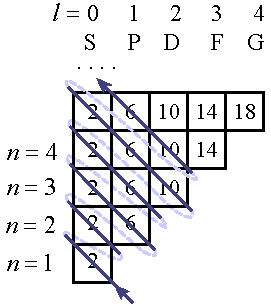
\includegraphics[width=4cm]{./figures/Ptable3.pdf}
\caption{轨道的填充顺序} 
\end{figure}

\subsection{元素周期表的排序}

要判断某个原子所在的周期, 就先根据原子序号找出上图中所有装有电子的格子, 其中 $n$ 最大的格子就是该元素所在的周期. 例如 30 号元素, 可以按照上图绿色线条的顺序占满 $1S, 2S, 2P, 3S, 3P, 4S, 3D$ (这些格子能容纳的总电子数刚好是 30). 其中 $4S$ 的主量子数最大,$n=4$, 所以 30 号元素在第四周期. 按照这个规律, 把上图按照周期分类如下.
\begin{figure}[ht]
\centering
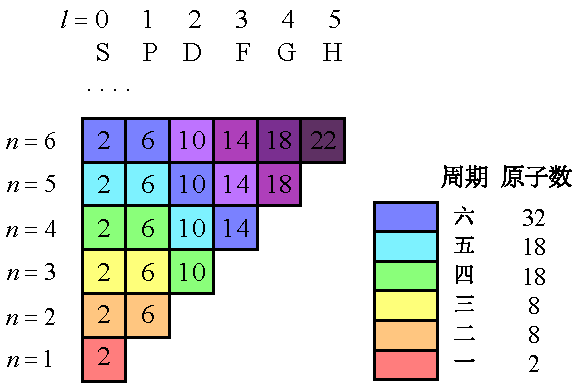
\includegraphics[width=8cm]{./figures/Ptable4.pdf}
\caption{划分周期} 
\end{figure}

